\documentclass[11pt,a4paper]{article}
\usepackage[margin=23mm]{geometry}
\usepackage{fontspec}
\setmainfont{TeX Gyre Termes}
\usepackage{booktabs,longtable,tabularx,array,amsmath,xcolor,fancyhdr,float}
\usepackage{tikz,pgfplots}
\pgfplotsset{compat=1.18}
\usetikzlibrary{arrows.meta,positioning,calc}
\usepackage[hidelinks]{hyperref}
\definecolor{ink}{HTML}{173E52}
\setlength{\parskip}{5pt}
\setlength{\parindent}{0pt}
\setlength{\emergencystretch}{3em}
\renewcommand{\arraystretch}{1.15}
\pagestyle{fancy}\fancyhf{}
\fancyhead[L]{\small bdd26 --- Stage report 6}
\fancyhead[R]{\small 26 October 2026}
\fancyfoot[C]{\thepage}
\setlength{\headheight}{15pt}
\newcommand{\src}[1]{\par{\footnotesize\color{gray}Evidence: #1}\par}
\title{\bfseries From Fitting Nuclei to Finding Them Reliably\\[8pt]\Large Nuclear instance segmentation: stage report 6}
\author{Xinhao Jin \quad Biomedical Data Design}
\date{Research period: 13--26 October 2026\\Evidence cutoff: 26 October 2026, 09:27 EDT}
\begin{document}
\maketitle
\begin{abstract}
Stage report 5 ended without a successful route from post-hoc typing or learned candidate quality to a qualified improvement. This stage moved the investigation upstream, into supervision, instance generation, and candidate detection. Three questions guided the work: can visibility-aware supervision repair crop-related failures; where do set-query models lose usable objects; and can a point detector produce reliable candidates before a mask model is introduced?

No completed method in this stage qualified for three-split confirmation. The experiments nevertheless separated several mechanisms that had previously been easy to conflate. Crop sensitivity was reproducible, but the tested supervision repair did not work. Query models produced some useful raw masks, then lost many objects through query retention and pixel competition. Point detectors could almost memorize the fitting images, yet their recall and precision on held-out images remained insufficient. More training, rare-class resampling, and restricted backbone adaptation did not resolve this problem under the tested recipes.

This report records both the negative results and the limited positive signals, with the evaluation population attached to each number. At the cutoff, P16 had one fully verified seed; its other seed was incomplete. P17 had passed implementation and real-V100 validation and had been submitted as a new, independently specified comparison of a convolutional pyramid detector with the existing UNI detector. Submission is a procedural milestone, not a performance result.
\end{abstract}

\begin{quote}\small
\textbf{Snapshot status.} P16 seed 19 was complete and checked; seed 1 C/R had reached epochs 85/73. P17 validation job 55297045 completed successfully. Production array \textbf{55297061} was submitted once at \textbf{09:08:19 EDT on 26 October}; all four tasks remained pending at the 09:27 cutoff.
\end{quote}
\newpage
{\small\tableofcontents}
\newpage

\section{Scope and the change in research question}

The previous stage chiefly asked whether existing features could support a better decision about nuclear type. The present stage asked an earlier question: without access to ground-truth locations, can a model first generate a sufficiently complete and precise collection of objects, then turn those objects into dependable instance masks? This matters for the Dead class, for crowded-instance separation, and for tissue-dependent robustness. Throughout this report, \emph{Dead} retains the dataset's category name. It includes apoptosis- and necrosis-related nuclei and is not synonymous with apoptosis alone.

The distinction between representation, detection, and final instance quality is central. A model may contain enough information to fit a mask when supplied with a true location. It may still fail to produce that location at inference. A query may generate a partially correct mask but be classified as background. A point detector may recall many centers while generating too many false candidates. These are different failures and require different evidence.

\begin{table}[H]\centering\small
\begin{tabularx}{\linewidth}{p{28mm}XX}
\toprule Study & Principal evidence & Current decision\\\midrule
Visibility supervision & Controlled crop audit; four training arms, two seeds & Sensitivity established; tested repair rejected\\
Set-query segmentation & Full E6/E7 training; object-level output tracing & Severe quality loss; slower decay did not recover it\\
High-resolution adaptation & Two-seed E19 comparison; shared failure set & Tested single-skip residual adapter did not repair interior Dead recall\\
Point detection & P1-R1 and P3--P15 fitting/audit contrasts & Strong fitting did not yield qualified generalization\\
Latest work & One complete P16 seed; P17 validation and submission & P16 incomplete; P17 has no production outcome yet\\
\bottomrule
\end{tabularx}
\caption{Research decisions at the fixed evidence cutoff.}
\end{table}

\subsection{Three evaluation settings}

Full segmentation development studies trained on fold1 and evaluated on fold2. Their metrics include mPQ, which incorporates instance matching, shape, and type; bPQ, which ignores type; and strict Dead PQ, which also penalizes Dead false positives on images without that class. They measure final segmentation behavior.

The later point studies used an image-level fitting/audit partition within fold1. A predicted center had to match a ground-truth center uniquely within three native-image pixels. This measures candidate localization, not mask contour quality. Point recall therefore cannot be subtracted from an IoU-based mask matching rate to estimate a pipeline loss.

Training diagnostics sometimes supplied true points, correspondences, or ground-truth-based selection of the best query. These experiments test whether a representation or readout can fit a restricted task. Such assistance is unavailable during ordinary inference. Their high values are useful mechanistic evidence, but not performance on unseen images.

All admission decisions retain their original endpoints and quality constraints. Failure means that the complete prespecified condition was not met; it does not mean that every metric decreased. Repeated experiments on the same images are also not independent statistical votes.

\subsection{Related class-merging audit}

An Inf/Conn class-merging audit was also completed. In the merged label space, the official metric increased by approximately .0519 and the gap to the ideal-classification upper bound narrowed by about 35.2\%. Merging labels mechanically removes some errors, so this is not an estimate of the loss caused by biological label ambiguity. The five-class method scores remain unchanged.

\src{Stage report 5; 15 October research synthesis; 18 October E-series review; P3--P15 progress synthesis. Historical results were checked against the current saved documents, rather than rerunning every historical model.}

\section{Visibility: a reproducible vulnerability without a successful repair}

\subsection{What the corrected crop audit established}

E4 first compared nuclei touching the original image boundary with interior nuclei, then applied controlled crops to nuclei that had originally been complete. In the corrected analysis, the area-stratified excess Dead miss rate for original boundary objects over interior objects was $+.1738$, with a 95\% interval of $[.1060,.2528]$. The controlled-crop difference-in-differences was $+.1474$, whereas the interpolation control was approximately $-.0006$.

The newly truncated fragments showed a large size-associated difference. Fragments smaller than 30 native pixels had a miss rate .8175 higher than objects of at least 100 pixels, with interval $[.7968,.8393]$. These findings support crop-related fragility as a real research target.

The audit required a correction. Its early version included inference in training mode and an unstratified decision. The valid basis is the corrected 14 October output. The corrected result still does not establish that zeroed horizontal/vertical (HV) targets are the sole cause: cropping changes both visible area and surrounding context.

\subsection{Full training of four supervision recipes}

The next study compared A0, the original training recipe; A1, crop augmentation; A2, crop augmentation with selective HV supervision; and A3, broader supervision for small targets. Each arm used two seeds and 130 epochs. Evaluation used the last checkpoint on both original images and fixed cropped images.

\begin{table}[H]\centering\small
\begin{tabular}{lrrrr}\toprule
Two-seed mean difference & mPQ & bPQ & Dead PQ & Strict Dead PQ\\\midrule
A1$-$A0 & $-.005284$ & $-.006122$ & $+.037648$ & $+.008833$\\
A2$-$A0 & $-.006269$ & $-.005438$ & $+.024565$ & $-.000948$\\
A2$-$A1 & $-.000985$ & $+.000685$ & $-.013083$ & $-.009781$\\\bottomrule
\end{tabular}
\caption{Development results on original fold2 images. Means summarize the two fixed seeds; they do not establish significance by themselves.}
\end{table}

A1 produced a positive Dead signal at a cost to overall segmentation quality. A2 did not remove that cost. Compared with A1, both Dead PQ and strict Dead PQ decreased in both seeds. The original-image quality constraint failed.

The more direct crop-mechanism test was supported by 116 eligible Dead objects from 38 images. Defining A1$-$A2 miss-rate change so that a positive value favors A2, the two seeds gave $-.025862$ and $+.008621$. Their mean was $-.008621$, with a 95\% interval of $[-.040918,+.017699]$. The selective-supervision treatment did not demonstrate the required reduction in misses.

The resulting decision is specific: crop sensitivity is supported, while this selective-supervision repair is not. The vulnerability does not validate the proposed remedy, and rejection of the remedy does not rule out every visibility-aware training method.

\src{E4 visibility probe, corrected 14 October; visibility-supervision development and mechanism records, 15 October.}

\section{Set-query segmentation: losses along the instance-generation chain}

\subsection{Full training revealed a broad quality collapse}

E6 compared the dense segmentation baseline B with query-mask model Q under matched conditions. E7 then changed the learning-rate decay factor from .85 to .99 to test whether excessively rapid decay could explain the result. Each round comprised two arms and two seeds, each trained for 130 epochs on fold1, with fold2 used for development evaluation.

\begin{table}[H]\centering\small
\begin{tabular}{llrrrr}\toprule
Round & Model & mPQ & bPQ & Dead PQ & Merge rate\\\midrule
E6 & B: dense baseline & .481432 & .650773 & .179635 & .045363\\
E6 & Q: query masks & .102699 & .192614 & .005951 & .285885\\
E7 & B: dense baseline & .472939 & .650651 & .131493 & .051209\\
E7 & Q: query masks & .087958 & .169912 & .006287 & .219744\\\bottomrule
\end{tabular}
\caption{Two-seed means within each round. Comparisons require the corresponding same-round baseline.}
\end{table}

Q underperformed B on all five class PQ values and on mPQ in all 19 tissues. Interior Dead matching at IoU$>.5$ decreased by .507422 in E6 and .528340 in E7; both corresponding intervals lay entirely below zero. The slower schedule did not restore basic instance quality. Although the cost condition passed, that did not compensate for the quality failure.

The models were not simply blind to every nucleus. In E6, the fraction of interior Dead objects with IoU between .1 and .5 rose from approximately 9.99\% to 55.60\%. Many objects had partial overlap without becoming qualified instances. This implicates localization, contour formation, and separation as well as complete misses.

\subsection{Tracing usable raw masks to final objects}

For the same 16 training images and 331 targets in E7, the analysis searched all queries for the best overlap with each target, rather than examining only its training-assigned query. This reveals what was present in the raw masks and where it was subsequently lost.

\begin{figure}[H]\centering
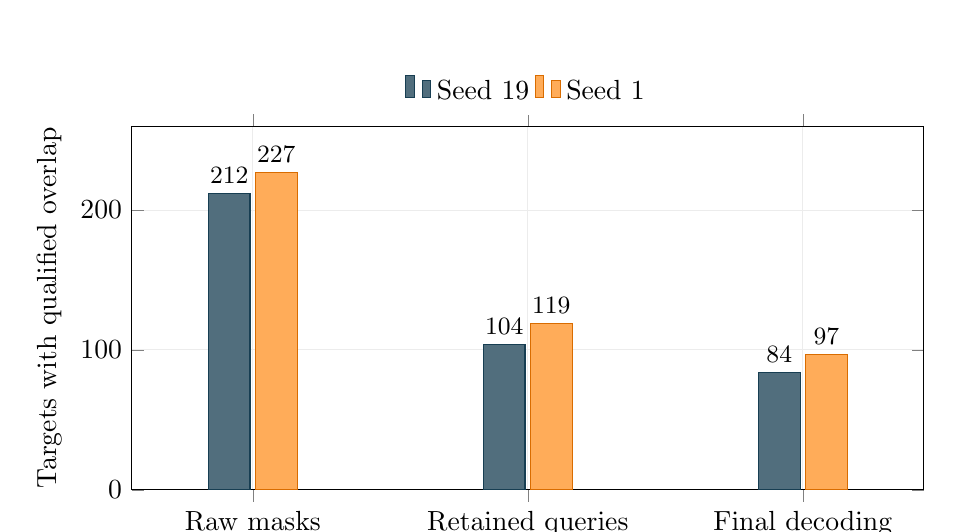
\begin{tikzpicture}
\begin{axis}[width=.96\linewidth,height=62mm,ybar,bar width=15pt,
ymin=0,ymax=260,ylabel={Targets with qualified overlap},
symbolic x coords={Raw masks,Retained queries,Final decoding},xtick=data,
legend style={at={(.5,1.03)},anchor=south,legend columns=2,draw=none},
nodes near coords,nodes near coords style={font=\small},
enlarge x limits=.22,grid=major,grid style={gray!15}]
\addplot[fill=ink!75,draw=ink] coordinates {(Raw masks,212) (Retained queries,104) (Final decoding,84)};
\addplot[fill=orange!65,draw=orange!85!black] coordinates {(Raw masks,227) (Retained queries,119) (Final decoding,97)};
\legend{Seed 19,Seed 1}
\end{axis}
\end{tikzpicture}
\caption{E7 object attrition on a fixed training batch. The all-query raw-mask stage uses ground truth to choose the best overlap and provides a ground-truth-assisted raw-mask coverage diagnostic. Qualified-object sets need not be nested across stages.}
\end{figure}

For seed 19, 212 targets passed the raw-mask criterion, 104 remained represented among retained queries, and final decoding qualified 84. Seed 1 gave 227, 119, and 97. Query retention lost 108 of 331 targets in each seed, or 32.63 percentage points. Pixel competition introduced a further net loss of about six percentage points.

Lowering a confidence threshold alone cannot undo rejection by a background argmax. Moreover, even the raw-mask coverage was only about 64--69\%. The failure therefore cannot be assigned entirely to one final threshold. Learning a mask, deciding which queries represent objects, and resolving overlapping pixels need separate checks before more training is justified.

\src{Set-mask E6 development, 16 October; set-mask E7 development, 17 October; associated fixed-batch diagnostics.}

\section{Small diagnostics separate representational capacity from inference}

E8--E18 investigated classification readout, query initialization, attention, auxiliary supervision, and object correspondence before committing to another full model. Their principal value was to test concrete repairs and to distinguish fitting with true-object assistance from finding objects autonomously.

\small
\begin{longtable}{p{18mm}p{43mm}p{89mm}}
\toprule Study & Intervention or diagnostic & Result and interpretation\\\midrule\endhead
E8 & Frozen features; classification-readout changes & Foreground fitting accuracy reached approximately 95--98\%, but foreground decisions deteriorated on held-out images and the assignment condition failed. A better fitted classifier did not yield a reliable instance set.\\
E9 & Queries initialized from local content & A small point-estimate gain in Dead geometric recall came with lower precision. Neither seed qualified.\\
E10 & Predicted-mask-constrained attention & Interior Dead changes were $-.067511/+.008439$ across the two seeds; overall recall also decreased.\\
E11 & Four-stage auxiliary supervision & Both the original assignment condition and the independent A0 constraint failed. The fixed recipe was stopped.\\
E12/E13 & Ground-truth-assisted free coefficients or stable projection & E12 fitted Dead at 86.32\%/87.37\%, demonstrating capacity under assisted conditions. Freezing the E13 projection still failed the quality conditions.\\
E14 & Exact native-resolution matching & Exact matching was implemented, but assignment and A0 constraints remained unmet. More accurate matching did not establish an effective method.\\
E15/E16 & True-point readout and point-conditioned masks & E16 GT-point-conditioned raw-mask coverage (IoU $>.5$) for fitted Dead reached 84.21\%/80.26\%; readout-held-out images gave 31.58\%/42.11\%. The frozen E7 model had previously seen these images, so this was not independent generalization of the entire model.\\
E17 & Sparse predicted points as candidates & No candidates were emitted in the fixed training diagnostic. The current recipe failed.\\
E18 & Dense voting as candidates & Excess candidates produced final-instance audit precision of only about 3.5--3.7\%. This is a different endpoint from P3's three-pixel point precision.\\\bottomrule
\end{longtable}
\normalsize

These studies reused small cohorts and serve as mechanism diagnostics. E6/E7 already supplied full-training negative evidence, so insufficient training is not a sufficient explanation of the query results. Conversely, the assisted fitting in E12/E16 makes a claim of no representational capacity too strong.

The next research requirement was therefore more elementary: demonstrate recall, precision, and cross-image transfer for genuinely predicted candidates before attaching a mask generator.

\src{E8 query-mechanism study; E9--E16 individual diagnostic records; E17/E18 and 17 October query/point closeout.}

\section{Gated fusion and high-resolution adaptation}

\subsection{A PQ gain did not establish recovery of missed objects}

E5 gated fusion increased official Dead PQ by .017897 and strict Dead PQ by .014202 on average. Interior Dead geometric matching, the chosen primary target, changed by $-.003374$, with interval $[-.014273,+.007486]$.

The composition and typing of matched objects changed. It would be inaccurate to attribute the entire PQ gain to missing-class evaluation rules, but equally inaccurate to interpret it as successful recovery of missed objects. Because the primary target failed, this recipe was not expanded.

\subsection{E19 tested a specific residual adapter}

E19 inserted a zero-initialized CNN residual branch into the finest decoder skip of CellViT-UNI. Across four full training runs, interior Dead matching changed by $-.008097$, with interval $[-.022566,+.007378]$. Official Dead PQ decreased by .001774 on average; strict Dead PQ rose by .008128. The main condition still failed.

This was a test of one insertion point, structure, and training budget. It was neither a reproduction of every multiscale adaptation method nor a refutation of earlier observations from increasing working resolution.

\subsection{The persistent failure set}

Among the same 741 interior Dead objects, 233 failed to reach IoU$>.5$ under all four models: 31.44\%. A smaller set of 149, or 20.11\%, had IoU$<.1$ in all four. The larger set includes roughly localized objects whose shape or separation remained inadequate and should not all be called complete misses.

Of the 233 persistently unmatched objects, 176 had area below 100 native pixels; their median area was 64. The four-model matching union covered 508 of 741 objects, only 37 more than the strongest individual model's 471. This union uses truth to select successful matches and does not resolve false positives or conflicts. It describes remaining coverage potential, not a deployed ensemble.

\begin{table}[H]\centering\small
\begin{tabular}{lrrr}\toprule
Area group defined on training fold & Training objects & Development objects & Unmatched by all four\\\midrule
$<67$ & 200 & 179 & 123 (68.7\%)\\
67--102 & 196 & 209 & 55 (26.3\%)\\
103--157 & 204 & 189 & 20 (10.6\%)\\
$\ge158$ & 201 & 164 & 35 (21.3\%)\\\bottomrule
\end{tabular}
\caption{Descriptive groups for the fixed object cohort. Area boundaries were established from the training fold, not selected from development failures.}
\end{table}

All 16 combinations of area and local-contrast bins had training support, and the marginal training/development medians were similar. Thus a simple absence of the relevant sizes or contrast ranges from training is not sufficient to explain the failures. Joint shifts involving tissue, appearance, and unknown patient factors remain possible. Small area is strongly associated with failure, but larger objects also fail persistently.

Tissue support is particularly uneven. Lung contributes 535 of these 741 interior Dead objects and Colon contributes 83. This denominator differs from the whole-dataset statistic that Lung contains 59.5\% of Dead labels. Seven tissues have no Dead labels; a lack of evaluable objects is not evidence of strong performance.

\src{Fusion-gating development; E19 high-resolution adapter development; 18 October E-series review and research decision; 15 October tissue/class audit.}

\section{Point detection: fitting images is easier than transferring to new images}

\subsection{P1-R1 tested the insufficient-training explanation}

The initial frozen-feature point head emitted no candidates under its short budget. Training was extended under a previously fixed training-loss stopping rule. The two seeds reached 55 and 60 epochs, approximately 94--98\% training recall and 99.9\% training precision.

On fold2, however, interior Dead point recall was only .40756/.39541, below the fixed NP-component candidate reference of .74899. Both seed-specific difference intervals lay below zero. Better fitting did not make the detector generalize, so the prerequisite for proceeding from P1 to P2 was not met. The NP-component result is a point-candidate reference, not mask IoU or official PQ.

\subsection{P3 separated adaptation from augmentation}

P3 fixed an image-level partition within fold1: 2,134 fitting images and 522 audit images. Only 11 audit images contained interior Dead objects, totaling 145; Lung and Colon together contributed 116. All arms used native-image center targets and fixed decoding. Frozen versus adapted UNI and absent versus present augmentation formed four combinations, each trained for two seeds and 130 epochs.

\begin{table}[H]\centering\small
\begin{tabular}{lrrrr}\toprule
Arm & Fitting recall & Audit recall & Audit precision & Audit Dead recall\\\midrule
F0: frozen, no augmentation & .999922 & .442776 & .706998 & .351724\\
F1: frozen, augmentation & .538848 & .428857 & .815171 & .396552\\
T0: adapted, no augmentation & .999833 & .509918 & .724614 & .375862\\
T1: adapted, augmentation & .977035 & .588939 & .692705 & .437931\\\bottomrule
\end{tabular}
\caption{Arithmetic means of the two fixed seeds in P3. All endpoints are point matching.}
\end{table}

Without augmentation, both representations nearly memorized the fitting images. With augmentation, the frozen representation itself became hard to fit; adaptation recovered much of that fit. T1 exceeded F1 in overall audit recall by about 16 percentage points, but lost about 12.25 percentage points of precision. Interior Dead gains were 6.90 and 1.38 percentage points in the two seeds, with intervals crossing zero in both.

This is a real recall/precision tradeoff rather than an unqualified improvement. It also shows why high training recall is insufficient: even T1's strong fit did not produce the required audit behavior.

\subsection{The fixed admission rule}

Each seed separately had to satisfy all of the following: interior Dead recall at least .60; gain over its corresponding control at least .05; a positive lower bound from the original tissue-stratified image bootstrap; unique-match precision at least .75 and no more than .02 below control; overall recall no more than .02 below control; and the original support and nondegeneracy conditions.

The rule is a research decision constraint, not a claim of ideal statistical power. Eleven positive audit images provide limited support, and repeated inspection of the same audit set further limits confirmation. Keeping the rule fixed prevents a favorable isolated seed or metric from becoming a retrospective justification for expansion.

\src{P1-R1 result, 18 October; P3 Phase A, 20 October; original admission implementation.}

\section{P4--P15: fixed interventions and their distinct failure patterns}

Subsequent rounds retained the cohort, seeds, 130-epoch schedule, last-checkpoint evaluation, and admission criteria. Each introduced a fixed recipe and retrained a same-round control. The table reports treatment minus that control. It is not a ranking of treatments from different rounds.

\begin{table}[H]\centering\small
\begin{tabularx}{\linewidth}{p{11mm}Xrr}\toprule
Round & Fixed intervention & Seed 19 & Seed 1\\\midrule
P4 & Dense foreground auxiliary BCE & $-.027586$ & $+.006897$\\
P5 & Equal-capacity native-grid refinement & $.000000$ & $-.006897$\\
P6 & Broader Gaussian-neighborhood negative-loss suppression & $+.020690$ & $+.020690$\\
P7 & Training-time RGB channel perturbation & $+.034483$ & $-.013793$\\
P8 & Loss normalization by object count within each image & $-.034483$ & $-.048276$\\
P9 & Dead-center positive-loss weight of 4 & $+.006897$ & $+.048276$\\
P10 & Adapt only the last 4 backbone blocks instead of 12 & $+.027586$ & $-.013793$\\
P11 & Redistribute positive focal mass at exact centers & $+.041379$ & $.000000$\\
P12 & Channel dropout .2 after the decoder stem & $-.034483$ & $-.027586$\\
P13 & Replace 25\% of training slots with rare-class-positive images & $-.137931$ & $-.048276$\\
P14 & Reduce encoder learning rate from $10^{-5}$ to $10^{-6}$ & $-.068966$ & $-.089655$\\
P15 & Integer translation up to $\pm16$ pixels, white padding & $-.193103$ & $-.089655$\\\bottomrule
\end{tabularx}
\caption{Interior Dead point-recall changes. None of P4--P15 met the original admission condition.}
\end{table}

\begin{figure}[H]\centering
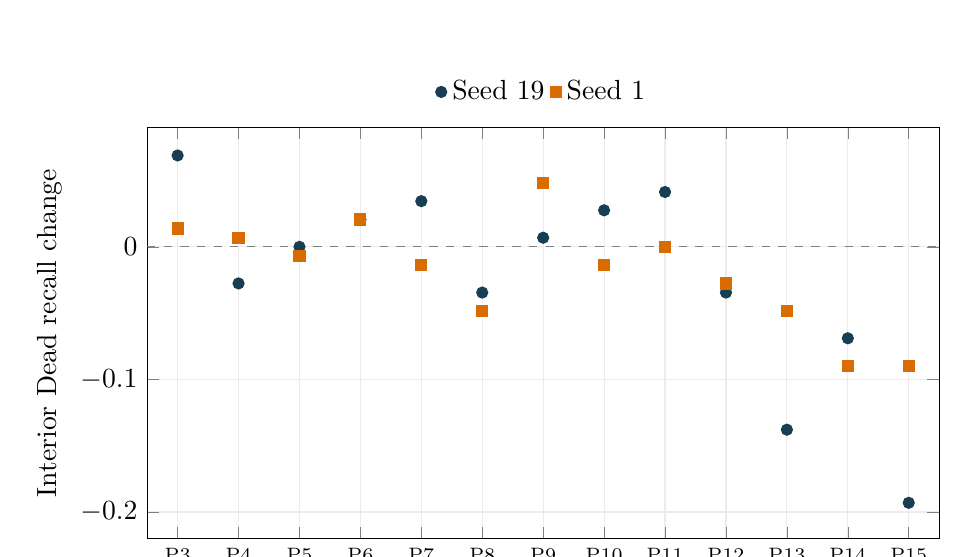
\begin{tikzpicture}
\begin{axis}[width=.96\linewidth,height=68mm,xmin=2.5,xmax=15.5,
ymin=-.22,ymax=.09,xtick={3,...,15},xticklabels={P3,P4,P5,P6,P7,P8,P9,P10,P11,P12,P13,P14,P15},
xticklabel style={font=\scriptsize},ylabel={Interior Dead recall change},
grid=major,grid style={gray!15},
legend style={at={(.5,1.03)},anchor=south,legend columns=2,draw=none}]
\addplot[ink,only marks,mark=*] coordinates {(3,.068966)(4,-.027586)(5,0)(6,.020690)(7,.034483)(8,-.034483)(9,.006897)(10,.027586)(11,.041379)(12,-.034483)(13,-.137931)(14,-.068966)(15,-.193103)};
\addplot[orange!85!black,only marks,mark=square*] coordinates {(3,.013793)(4,.006897)(5,-.006897)(6,.020690)(7,-.013793)(8,-.048276)(9,.048276)(10,-.013793)(11,0)(12,-.027586)(13,-.048276)(14,-.089655)(15,-.089655)};
\addplot[gray,dashed,forget plot] coordinates {(2.5,0)(15.5,0)};
\legend{Seed 19,Seed 1}
\end{axis}
\end{tikzpicture}
\caption{Chronological P3--P15 point estimates. P3 denotes T1$-$F1; later rounds denote treatment minus a newly trained control. These estimates are not significance tests or a hyperparameter ranking.}
\end{figure}

\subsection{Strong fitting with weak transfer}

P13 increased exposure to rare-class-positive images. Its fitting Dead recall reached .998476/1, whereas audit Dead recall was .351724/.358621. Within this recipe, more repeated exposure did not lead to transfer. The explanation that the model simply had not seen the rare examples often enough is therefore insufficient.

The result does not show that class imbalance is irrelevant. It shows that this fixed resampling intervention, at this budget and with this representation, did not solve it. Fitting and transfer need separate evidence even when the intervention targets a plausible data imbalance.

\subsection{Restricting adaptation did not restore the required balance}

Training fewer backbone blocks, adding dropout, and reducing backbone learning rate all failed admission. P14 increased precision but reduced overall recall by approximately 8.83/12.01 percentage points. The detector became more selective while covering fewer objects. Precision alone would give a misleading account of its usefulness as a candidate generator.

\subsection{Augmentation can also impair fitting}

P15 is different from P13. On unaugmented fitting images, overall recall dropped from approximately .978 to .470 and interior Dead recall from approximately .952 to .45. The treatment made the fitting task itself much harder.

Integer translation jointly changed white borders, partially visible nuclei, position-invariance demands, and target visibility: approximately 9.94\% of center targets moved outside the image each epoch. Consequently, this round cannot isolate positional encoding as the cause.

Audit precision rose from .692/.698 to .865/.863, but candidate counts fell from 10,469/10,428 to 5,498/5,397. Unique matches also fell, from 7,241/7,280 to 4,758/4,657. Both seed-specific intervals for the Dead recall difference were entirely negative. The 512-candidate cap was never reached, so truncation by that cap is not supported as an explanation.

The three failure patterns give concrete stopping reasons for the tested recipes and distinct targets for subsequent diagnosis.

\src{Individual P4--P15 result records; proposal progress, 26 October. The summary rows were cross-checked against the saved result documents; all historical large checkpoints were not independently rehashed.}

\section{P16: full Gaussian regression, with only one completed seed}

\subsection{What changed}

In the original focal loss, only an exact center is positive; Gaussian neighborhood values reduce nearby negative loss. P16 retained target geometry but directly minimized the sum of squared differences between sigmoid outputs and the Gaussian target, divided by the valid-batch object count, with coefficient fixed at 1.

This changes gradients, background weighting, and loss scale together. A result cannot therefore be interpreted as an isolated test of Gaussian neighborhood supervision or probability calibration.

\subsection{Verified seed-19 result}

At the first recovery, both seed-19 arms had completed 130 epochs with SLURM state COMPLETED/0:0. Eighteen small result files matched their stored sizes and SHA256 values; 401 archived source files were checked individually. Fitting/audit identities, epoch logs, and per-image aggregation were also checked.

\begin{table}[H]\centering\small
\begin{tabular}{lrr}\toprule
Seed 19 endpoint & C: original focal & R: Gaussian regression\\\midrule
Fitting overall recall & .980007 & .872135\\
Fitting interior Dead recall & .961890 & .846037\\
Audit overall recall & .598041 & .602531\\
Audit unique-match precision & .694079 & .701149\\
Audit interior Dead recall & .482759 & .517241\\\bottomrule
\end{tabular}
\caption{P16 last-checkpoint point results for the completed seed only.}
\end{table}

The Dead gain was $+.034483$, corresponding to five additional matched objects. Replaying the original 1,000 tissue-stratified image bootstrap draws gave a 95\% interval of $[-.034091,+.131144]$. The seed failed the original rule: absolute recall remained below .60, gain below .05, the interval crossed zero, and precision remained below .75.

At the first recovery, seed 1 was still running, with C/R at epochs 70/58; the final 09:27 EDT snapshot recorded 85/73. Neither arm had completed at the cutoff. A two-seed mean or complete closeout would therefore be premature. Even a favorable second seed could not erase failure of a rule that must pass separately in each seed. Large checkpoints were not independently rehashed in this round, and external archiving remained pending.

\src{Recovered P16 seed-19 small-file package; stored manifest; per-image records; original gate and bootstrap replay.}

\section{P17: an independently specified convolutional detector comparison}

\subsection{Question and controlled boundaries}

P17 was fixed before P16 seed 1 finished and does not depend on its incomplete outcome. Control C retains the existing UNI detector. Treatment K trains a three-stage convolutional pyramid from scratch, with widths 32/64/128, multiscale fusion, and native-center heatmap output. It does not add queries, masks, rare-class resampling, or extra supervision.

Both arms retain the same fitting/audit cohorts, original focal loss, Gaussian targets, augmentation, fixed decoding, and admission rule. K uses learning rate $3\times10^{-4}$ for all parameters. C retains $3\times10^{-4}$ for its head and $10^{-5}$ for its backbone.

This is a practical comparison of recipes that differ in architecture, initialization, pretraining, and optimization. It is not a causal isolation of locality. GroupNorm also uses spatial statistics, so K is not a strictly finite-receptive-field local operator.

The decision question is whether this from-scratch convolutional representation merits further work within the original budget. Failure closes this width, schedule, and loss combination without expanding widths, seeds, thresholds, or epochs. Passing would justify discussing another validation plan; it would not automatically authorize masks or three-split confirmation.

\subsection{Implementation validation and submission receipt}

Real-V100 validation job 55297045 completed on exp-7-59 with state COMPLETED/0:0 in 6 minutes 12 seconds; 291 node checks passed. For both seeds, control initialization and the complete two-step gradients, parameters, AdamW state, and random state agreed with P3. K's three convolutional stages, fusion head, and output layer all had nonzero second-step gradients and updates; pure weight decay was excluded as their explanation.

AMP behavior, last/final checkpoint reloads, source/data identity, and strict readiness passed. Twenty-five small evidence files were checked for size and SHA256 on recovery.

With a 1.5 safety multiplier, extrapolated 130-epoch time was 6.95 hours for C and 4.77 hours for K. Training peak GPU memory was approximately 4.07/.35 GiB. These are resource estimates, not completion guarantees.

\begin{table}[H]\centering\small
\begin{tabularx}{\linewidth}{p{42mm}X}\toprule
Submission field & Recorded value\\\midrule
Production array & 55297061; submitted once, 26 October 2026, 09:08:19 EDT\\
Task order and concurrency & C19, K19, C1, K1; at most two concurrent tasks\\
Per-task request & One V100, four CPUs, 32 GiB RAM, 12 hours\\
Partition, QoS, account & gpu-shared; gpu-shared-normal; jhu159\\
Filesystem and restart policy & Lustre; automatic requeue disabled\\
Maximum production budget & 48 GPU hours; validation separately capped at .5 GPU hours\\
Source identity & Commit \texttt{5a7e85b}; 407-file source archive\\
Initial scheduler state & All four tasks pending at submission\\\bottomrule
\end{tabularx}
\caption{P17 procedural evidence available by the report cutoff. No production training outcome is included.}
\end{table}

\src{Frozen P17 design; real-V100 validation receipt; archived source and evidence manifest; single production submission receipt.}

\section{Research execution and compute migration}

Formal recent training moved to Expanse. The initial replica comprised 420 files, approximately 8.10 GB, whose sizes and hashes were checked on a compute node. Large files moved through official Globus. Later rounds reused this data replica, UNI weights, and the fixed environment, while separately archiving source, configurations, and submission receipts.

P3 runs interrupted by source-disk protection before migration preserved their checkpoints and completed without recomputing the six already completed items. This continuity matters because a migration should not silently change training provenance or mix reruns with original outcomes.

In the saved checks for this reporting round, LM1 and LM2 had no project training processes. LM1 had no available root-partition space and approximately 11 GB on the project disk; LM2 had approximately 784 MB on root and 1.9 GB on its project disk. No new training or large-checkpoint recovery was added there. Expanse allocation availability, GPU partition eligibility, and individual/project quotas were checked; unrelated existing jobs were preserved. These are dated observations, not assertions about current machine state.

P17 reused the persistent execution channel and existing Expanse ControlMaster without creating another authentication connection or changing proxy mode. Each submission used an exclusively created marker and recorded the job ID. If a submission result was uncertain, receipts and scheduler records were inspected rather than replaying the submission. Validation compute ran through SLURM; login-node actions were limited to lightweight inspection and submission.

P13--P16 and earlier review corrections were merged and published to master on 26 October, at baseline commit \texttt{f67ce20}. The complete CPU regression at that point passed 828 tests with three skipped. P17 was implemented on a separate branch. Its final complete CPU suite passed 861 tests with three skipped and 19,073 warnings from older dependency deprecations. Proposal-specific and node-specific checks each passed 291 tests. These counts correspond to different code versions or check scopes; the original receipts were retained.

\section{What the evidence supports and what remains open}

The strongest contribution of this stage is a more precise account of failure. It separates crop vulnerability from successful supervision repair, raw query masks from retained instances, and fitting images from transfer to held-out images. These separations provide a basis for choosing the next experiment instead of stacking previously unsuccessful components.

Several concrete claims are now supported. The corrected crop audit found a substantial vulnerability. The tested selective HV supervision did not repair it. Full query-mask training suffered broad instance-quality losses, and the slower decay schedule was insufficient. The tested single-skip adapter did not improve the chosen interior Dead endpoint. The point-detector studies showed substantial fitting capacity but no completed recipe meeting the joint recall, precision, and stability conditions.

The evidence does not establish that the problem is impossible or that a whole architecture family is unsuitable. E19 failures are associated with small area but are not explained solely by size. Coarse training support does not guarantee coverage of the joint distribution. High fitting recall shows image memorization capacity, not a transferable model of nuclear appearance. Expert review remains unavailable, and detector agreement is not a substitute for biological adjudication.

The immediate next step is to close out the remaining P16 runs under the original decision rule. P17 likewise requires verification of 130 epochs, provenance, input identities, configurations, and manifests before a seed-by-seed decision. Only genuinely predicted candidates meeting recall and precision requirements would justify discussing a mask head or joint training. If they fail, the appropriate output is a documented failure mode and stopping rationale, not a larger parameter menu on the same 11 positive audit images.

\subsection{Limits that must accompany the final research account}

Fold2 and the internal fold1 audit set have been reused across experiments. Images are not necessarily independent patients. Bootstrap intervals condition on the fixed trained models and available images; they do not describe the full distribution over training seeds. Dead labels are unevenly distributed across tissues, and some tissues offer no Dead evaluation support. This stage has no new official three-split test result.

These limitations affect interpretation, not just presentation. A sequence of development failures cannot be treated as a collection of independent confirmatory trials. Similarly, a favorable future point estimate on this audit set would still require a fresh validation plan. The human-expert review obligation retained from stage report 5 remains unresolved.

\clearpage
\appendix
\section{Evidence index and verification scope}

Historical numbers in this report synthesize the saved research documents and closeout records. They are not presented as new evaluations of every old checkpoint. P16 seed 19 received a deeper check in this round: per-image reaggregation, replay of the original bootstrap, cohort verification, and 130-epoch log checks. Source-summary hashes and recovered numerical evidence are retained in the accompanying \texttt{verified\_numbers.json}.

\begin{longtable}{p{31mm}p{121mm}}
\toprule Evidence group & Saved record family and purpose\\\midrule\endhead
Previous-stage boundary & Stage report 5 README under \texttt{docs/report/}; experiments through 12 October, report released 13 October.\\
Visibility & E4 visibility probe; visibility-supervision development; visibility-supervision mechanism. The corrected E4 output is dated 14 October.\\
Query segmentation & E6/E7 set-mask development; E7--E18 query/point closeout; individual mechanism diagnostics E8--E18.\\
Gating, small objects, tissue & Fusion-gating development; E19 high-resolution adapter; E-series review; CellViT/PMNet research decision; tissue/class audit.\\
Point candidates & P1-R1 result; P3 Phase A; individual P4--P15 results; proposal progress dated 26 October.\\
Latest experiments & P16 small-file recovery package and stored manifests; P17 frozen design, 291-check logs, real-V100 validation, and production submission receipt.\\\bottomrule
\end{longtable}

Machine paths, process IDs, and connection evidence remain in ignored operational notes. Historical process IDs are evidence, not authority for later process operations. Original data, weights, predictions, and checkpoints are preserved; external archiving of large artifacts remains incomplete.

Execution followed the saved project workflow and the \href{https://www.sdsc.edu/systems/expanse/user_guide.html}{SDSC Expanse user guide}, together with the contemporaneous account, partition, and quota checks. This report introduces neither a new literature ranking nor an unverified state-of-the-art claim.
\end{document}
